% La on a perdu tout le monde

\subsection{Shape of Occupied Space: Topological Data Analysis}
In this section we will now try to answer the questions that rose from clustering algorithms, using techniques from \textit{Topological Data Analysis} (TDA for short) basing ourselves on the Python library Gudhi by \newcite{Gudhi}. 
The idea behind TDA is to look at our set of samples for each case as a triangulation\footnote{A mesh, of sorts} homeomorphical to a riemannian manifold, and to compute invariants to compare with other manifolds. 
Here, we will compute the homology groups of our manifold. Homology groups are algebraic structures which capture the topological invariants of a space, for example, the number of connected components, the number of holes, the number of voids etc\ldots
However, since we only have a set of points for our manifold and not an actual triangulation, we will use simplicial complexes to build a topological space and compute its homology. 
Simplicial complexes are a generalisation in multiple dimensions of graphs:
The $k$-dimensional simplicial complex of a set $X = \left\{x_{0}, \cdots, x_{k}\right\}$ of points is its convex hull. The points in $X$ are called vertices and the simplices generated from subsets of $X$ are called faces of the complex. 
To compare two simplicial complexes, we will compare their persistence diagrams.
The persistence diagram of a simplicial complex is a $2D$-diagram of points representing the moment a simplex is added to the complex creating a \textit{hole} and the moment a simplex is added to the complex closing the \textit{hole}, as well as their dimension. 

There are multiple ways to construct simplicial complexes. 
We decided to use the Rips Complex\footnote{or Vietoris-Rips}, which is a form of generalisation of $\alpha$-neighbourhood graphs, that is, there is a simplex of dimension $k$ or $k$-simplex (a $1$-simplex is an edge, a $2$-simplex is a triangle, a $3$-simplex is a tetrahedron, etc\ldots) between any $k + 1$ nodes such that their set has diameter at most $\alpha$.

\begin{figure}[h]
    \centering
    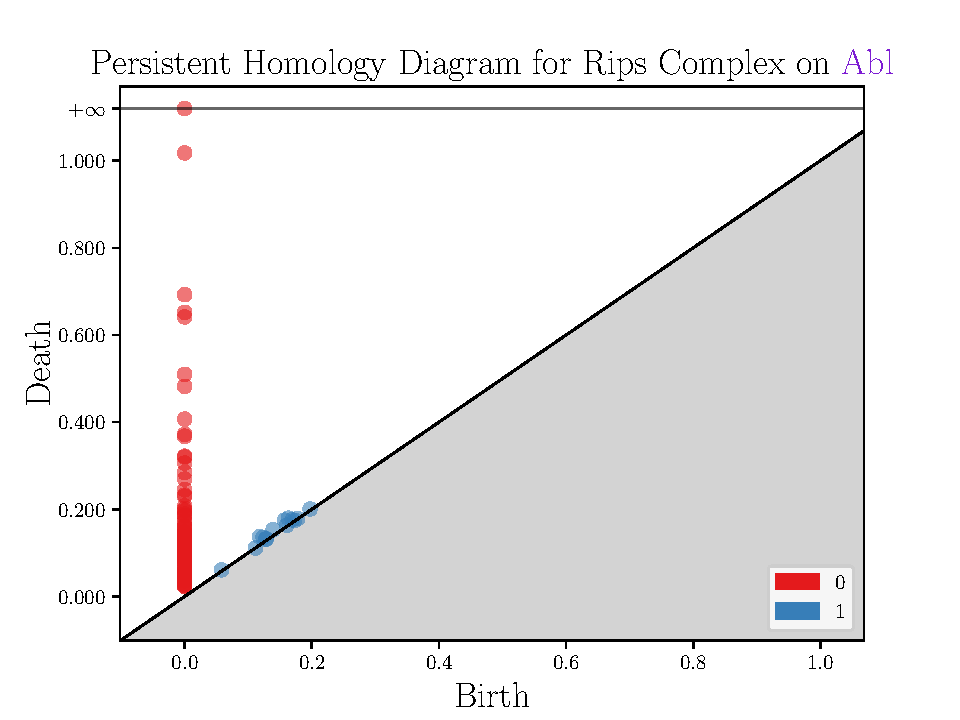
\includegraphics[width=\linewidth]{Images/rc_Abl.pdf}
    \caption{Persistence Diagram for the Rips Complex on the Ablative Manifold with $\alpha = 0.5$}
    \label{fig:rcabl}
\end{figure}

\begin{figure}[h]
    \centering
    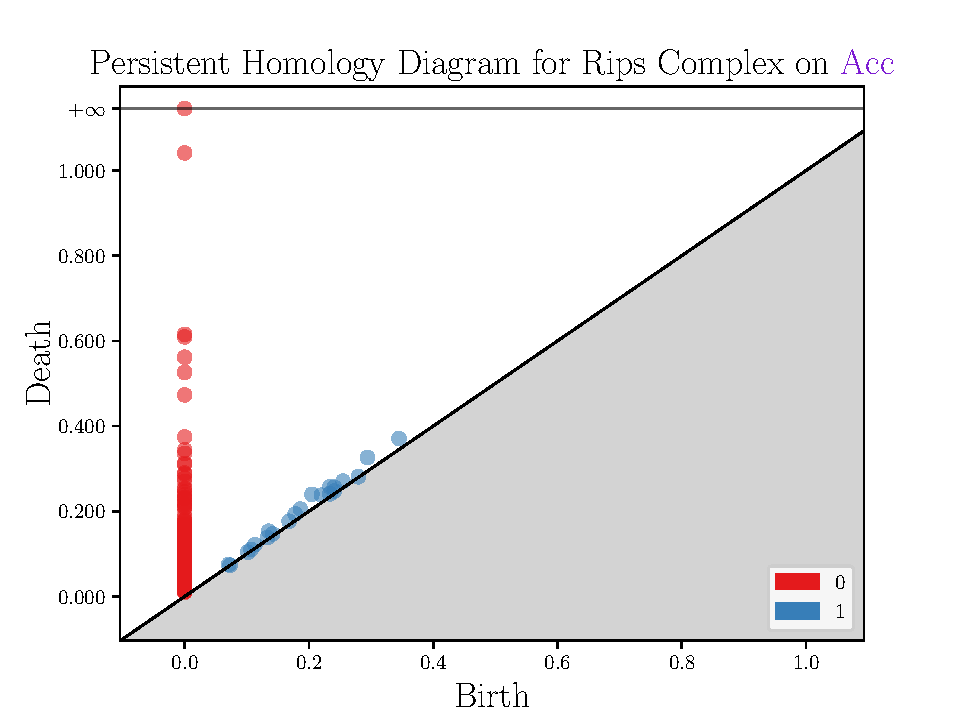
\includegraphics[width=\linewidth]{Images/rc_Acc.pdf}
    \caption{Persistence Diagram for the Rips Complex on the Accusative Manifold with $\alpha = 0.5$}
    \label{fig:rcacc}
\end{figure}

In figures \ref{fig:rcabl} and \ref{fig:rcacc}, we have computed the persistent homology diagram for Rips complexes on ablative and accusative manifolds. 
We can see a certain similarity between the graphs, especially in the number of connected components. 
This might indicate similarities in the shape of the representations/topology of the manifolds. 
To confirm our intuition we computed the Wasserstein $1$-distance between the diagrams, seen as tuples of distributions over the 2D space.

\begin{table}[h]
\centering
\addtolength{\tabcolsep}{-0.4ex}
\begin{tabular}{>{\tt}c|cccccc}
        \toprule
        Case & Abl & Acc & Dat & Gen & Loc & Nom\\
        \midrule
        Abl & \phantom{0.00} & 0.89 & 1.27 & 0.82 & 1.09 & 0.94\\
        Acc & 0.89 & \phantom{0.00} & 1.01 & 0.42 & 1.03 & 0.91\\
        Dat & 1.27 & 1.01 & \phantom{0.00} & 0.87 & 1.47 & 0.76\\
        Gen & 0.82 & 0.42 & 0.87 & \phantom{0.00} & 0.84 & 0.87\\
        Loc & 1.09 & 1.03 & 1.47 & 0.84 & \phantom{0.00} & 1.48\\
        Nom & 0.94 & 0.91 & 0.76 & 0.87 & 1.48 & \phantom{0.00}\\
        \bottomrule
\end{tabular}
\addtolength{\tabcolsep}{0.4ex}
\caption{Wasserstein $1$-distance between the Rips Complexes with $\alpha = 0.5$ of a few Cases}
\label{tab:wassrc}
\end{table}

Our results, presented in table \ref{tab:wassrc}, indicate that all the diagrams are quite close, given the number of points in each diagram, comforting us in the idea that spaces have similar shapes. 
While here the value of $\alpha$ seems arbitrary, we have tested for some other values, always with the same result, but the computing time made it quite difficult to perform extensive testing with many values. 
To reduce computing time, we tried using Čech complex, which is a sub-complex of the Rips complex created by adding $k$-simplices between sets of $k + 1$ points who were all at distance at most $\alpha$ of each other, but this provided equivalent results for the same computing time. 

This indicates that, as we thought, the manifolds for each case are quite similar in shape but are overlapping each other. This is consistent with the values seen when looking at the angles between different cases, which indicated that cases were in close yet different directions.